\section{Adaptive Sampling Strategies}
Performing UQ and Dynamic PRA can be
challenging from a computational point of view. The \textit{Forward}
sampling strategies reported in the previous Section can lead to a large number of
unnecessary evaluations of the physical model leading to an unacceptable resource expenses (CPU time).
In addition, the \textit{Forward} methodologies are not designed to leverage the information
content that is extractable from the simulations already concluded.

To overcome these limitations, in RAVEN several adaptive algorithms are available:
\begin{enumerate}
  \item \textit{Limit Surface Search}
  \item \textit{Adaptive Dynamic Event Tree}
  \item \textit{Adaptive Hybrid Dynamic Event Tree}
  \item \textit{Adaptive Sparse Grid}
  \item \textit{Adaptive Sobol Decomposition}.
\end{enumerate}
In this Section, only the first algorithm is going to be reported, explaining the theory behind it
and providing RAVEN examples.

%%%%%%%%%%%%%%%%%%%%%%%%%%%%%%%%
%%%%%%%%  Limit Surface Search %%%%%%%%
%%%%%%%%%%%%%%%%%%%%%%%%%%%%%%%%
\subsection{Limit Surface Search Method}
\label{sub:LS}
The motivation behind the choice of adaptive sampling strategies is that numerical
simulations are often computationally expensive, time consuming, and
with a large number of uncertain parameters. Thus, exploring the space
of all possible simulation outcomes is almost unfeasible using finite
computing resources. During DPRA analysis, it is
important to discover the relationship between a potentially large
number of uncertain parameters and the response of a simulation using
as few simulation trials as possible.
This is a typical context where ``goal'' oriented sampling could be
beneficial. The ``Limit
Surface Search method'' is a scheme  where few observations, obtained
from the model run, are used to build a simpler and computationally faster
mathematical representation of the model, ROM, also
known as Surrogate Model (ROM or SM). The ROM (see Section \ref{sec:ROMsTheory}) is then
used to predict where further exploration of the input space could be
most informative. This information is used to select new locations in the
input space for which a code run is executed (see
Figure~\ref{fig:ExampleLSschematic}). The new
observations are used to update the ROM and this process iterates
until, within a certain metric, it is converged.
\begin{figure}[h!]
  \centering
  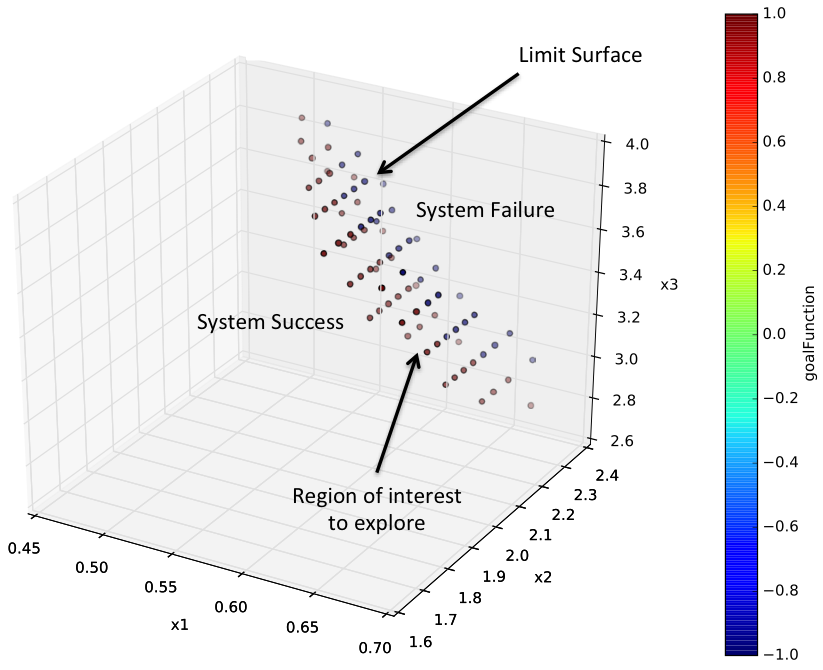
\includegraphics[width=1.0\textwidth]  {pics/ExampleLSschematic.png}
  \caption{Example of limit surface in the uncertain space.}
  \label{fig:ExampleLSschematic}
\end{figure}

In the case of the ``Limit
Surface (LS) Search method'', a ROM is used to
determine the location in the input space where further observations are most
informative to establish the location of the LS, then code runs are
executed on those locations and the ROM updated. The process
continues until the location of the LS is established within a certain tolerance.

%%%%%%%%%
%%%%%%%%% Limit Surface Concept and Properties
%%%%%%%%%
\subsubsection{Limit Surface Theory}
\label{sec:LSconcept}

To properly explain the LS concept and relative properties,
it is necessary to analyze the idea behind the LSs, firstly, from a
mathematical and, secondly, from a practical point of view.
Consider a dynamic system that is represented in the phase space by the Eq.~\ref{eq:dThetaOverDT} in Section~\ref{sec:RAVENconcept}.
The equation can be rewritten as follows:
\begin{equation}
\label{eq:ThetaXPT}
\frac{\partial \overline{\theta} }{\partial t}=\overline{H}\left (  \overline{x},\overline{p},t \right )
\end{equation}
where:
\begin{itemize}
  \item $\overline{\theta}$ represents the coordinate of the system in the
  phase space
  \item $\left (  \overline{x},\overline{p},t \right )$ independent variables
  that are separated, respectively, in spatial, temporal, and parametric
  space (distinction between $\left (  \overline{x},\overline{p},t \right )$ is purely based on engineering considerations).
\end{itemize}
Now it is possible to introduce the concept of ``goal'' function, $C$. $C$
is a binary function that, based on the response of the system, can
assume the value $0$ (false) to indicate that the system is properly
available (e.g., system success) and $1$ (true) to indicate that the
system is not available (e.g., failure of the system):
\begin{equation}
C\left (\overline{\theta}, \overline{x},\overline{p},t \right ) = C\left (H\left(\overline{x},\overline{p},t \right), \overline{x},\overline{p},t \right ) = C\left ( \overline{x},\overline{p},t \right )
\end{equation}
Without loss of generality, lets assume
that $C$ does not depend on time (e.g. $C\leftarrow
\bigintssss_{t_{0}}^{t_{end}}dtC\left(  \overline{x},\overline{p},t \right )$):
\begin{equation}
  \label{eq:goalFunction}
  C = C\left (\overline{x},\overline{p}\right )
\end{equation}
To simplify the mathematical description of the LS concept, it is
possible to hypothesize that the
equation describing the PDF time evolution of the system in the phase
space is of type Gauss
Codazzi (in its Liouville’s derivation)~\cite{MathFrameworkMC2013}, which allows ensuring that all the
stochastic phenomena in
the system are representable as PDFs in the uncertain domain
(see Section~\ref{sec:RAVENconcept}),. This allows combining the
parametric space with the initial condition space:
\begin{equation}
  \label{eq:goalFunctionCodazzi}
  \begin{matrix}
  \left ( \overline{x} \right ) \leftarrow \left ( \overline{x},\overline{p} \right ) \\
  C\left ( \overline{x} \right ) \leftarrow C\left ( \overline{x},\overline{p} \right )
  \end{matrix}
\end{equation}

This assumption is rarely violated, for example for those systems that
present an intrinsic
stochastic behavior (e.g., the dynamic of a particle of dust in the air
where it continuously and
randomly interacts with the molecules of air that ``move'' with different velocities and in different
and random directions). In most of the cases of interest in the safety analysis, the above
mentioned assumption is correct. The full heuristic approach to the characterization of system stochastic behaviors is reported in Section~\ref{sec:RAVENconcept}.
\\Under the above simplifications, it is possible to identify the region of the input space ($V$)
leading to a specific outcome of the ``goal'' function. For example, it can be defined
the failure region $V_{F}$ as the region of the input space where $C=1$:
\begin{equation}
 \label{eq:failureRegion}
V_{F}=\left \{ \forall \overline{x} | C\left ( \overline{x} \right ) = 1 \right \}
\end{equation}
The definition of the complementary of the failure region is obviously:
\begin{equation}
V_{F}^{c}=\left \{ \forall \overline{x} | C\left ( \overline{x} \right ) = 0 \right \}
\end{equation}
Its boundary is the named LS:
\begin{equation}
L_{S}= \partial V_{F}^{c}= \partial      \left \{ \forall \overline{x} | C\left ( \overline{x} \right ) = 1 \right \}
\end{equation}

The identification of the LS location is necessary to identify boundary regions for which the system under consideration will or will not exceed certain FOMs (e.g., operative margins).
\\The LS location is extremely important for design optimization and, in addition, its informative content can be used to analyze the system to characterize its behavior from a stochastic point of view. Consider $\overline{x} \in V$ and $\overline{x}\sim \overline{X}$,
where $\overline{x}$ is the random variate realization of the stochastic variable $\overline{X}$.
If $pdf_{\overline{X}}\left ( \overline{x} \right ) $ is the probability density function of $ \overline{X}$, the failure probability of the system $\left ( P_{F} \right )$ is:
\begin{equation}
\label{eq:probabilityFailure}
P_{F} = \bigintssss_{V}d\overline{x}C\left ( \overline{x} \right )pdf_{\overline{X}}\left ( \overline{x} \right ) = \bigintssss_{V_{F}+V_{F}^{c}}d\overline{x}C\left ( \overline{x} \right )pdf_{\overline{X}}\left ( \overline{x} \right )
\end{equation}
And, based on the definition given in Equations~\ref{eq:goalFunctionCodazzi} and \ref{eq:failureRegion}:
\begin{equation}
 \label{eq:failureProbIntegral}
 \bigintssss_{V_{F}}d\overline{x}pdf_{\overline{X}}\left ( \overline{x} \right )
 \end{equation}
Equations \ref{eq:probabilityFailure} and \ref{eq:failureProbIntegral} are summarized by stating that the system failure probability is
equivalent to the probability of the system being in the uncertain
subdomain (region of the input space) that leads to a failure pattern.
This probability is equal to the probability-weighted hyper-volume that is surrounded by the LS (see Figure ~\ref{fig:ProbabilityFailureLSExample}).
\begin{figure}[h!]
  \centering
  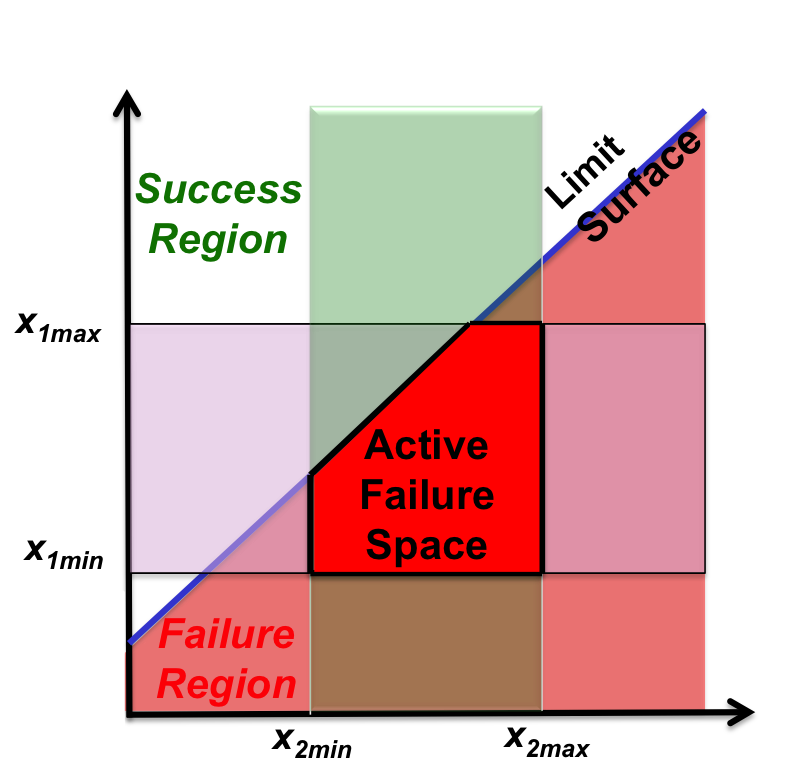
\includegraphics[width=1.0\textwidth]  {pics/ProbabilityFailureLSExample.png}
  \caption{Example of limit surface probability of failure region.}
  \label{fig:ProbabilityFailureLSExample}
\end{figure}
\\It is beneficial for better understanding to assess the LS concept through an example related to the safety of an Nuclear Power Plant (NPP).
As an example, consider a station black out (SBO) scenario in an NPP. Suppose that the only uncertain parameters are:
\begin{itemize}
  \item $t_{F}$: Temperature that would determine the failure of the fuel cladding
  \item $rt_{DGs}$: Recovery time of the diesel generators (DGs) that
  can guarantee, through the emergency core cooling system (ECCS),
  the removal of the decay heat.
\end{itemize}
And, the corresponding CDF (uniform) is:

\begin{equation}
t_{F}\sim pdf_{T_{F}}\left ( T_{F} \right )=\left\{\begin{matrix}
0 & if \: t_{F}< t_{F_{min}} \\
\frac{1}{\left ( t_{F_{max}}- t_{F_{min}} \right )=\Delta t_{F}} & \\
0 & if \: t_{F}>  t_{F_{max}}
\end{matrix}\right.
\end{equation}
%
%
\begin{equation}
rt_{DGs}\sim pdf_{RT_{DGs}}\left ( rt_{DGs} \right )=\left\{\begin{matrix}
0 & if \: rt_{DGs}<rt_{DGs_{min}}   \\
\frac{1}{\left ( rt_{DGs_{max}} - rt_{DGs_{min}} \right )=\Delta rt_{DGs}} & \\
0 & if \: rt_{DGs}>rt_{DGs_{max}}
\end{matrix}\right.
\end{equation}
For simplicity, assume that the clad temperature is a quadratic function of the DG recovery time in an SBO scenario:
\begin{equation}
  t = t_{0}+\alpha \times rt_{DGs}^{2}
\end{equation}
and that the  $ t_{F_{min}} > t_{0}+\alpha \times rt_{DGs_{min}}^{2}$
and $t_{F_{max}} < t_{0}+\alpha \times rt_{DGs_{max}}^{2}$.
The LS, failure region, and active part of the failure region (failure region with non-zero probability) are illustrated, for example, in Figure~\ref{fig:ProbabilityFailureLSExample} (in agreement with the above assumptions).
\begin{figure}[h!]
  \centering
  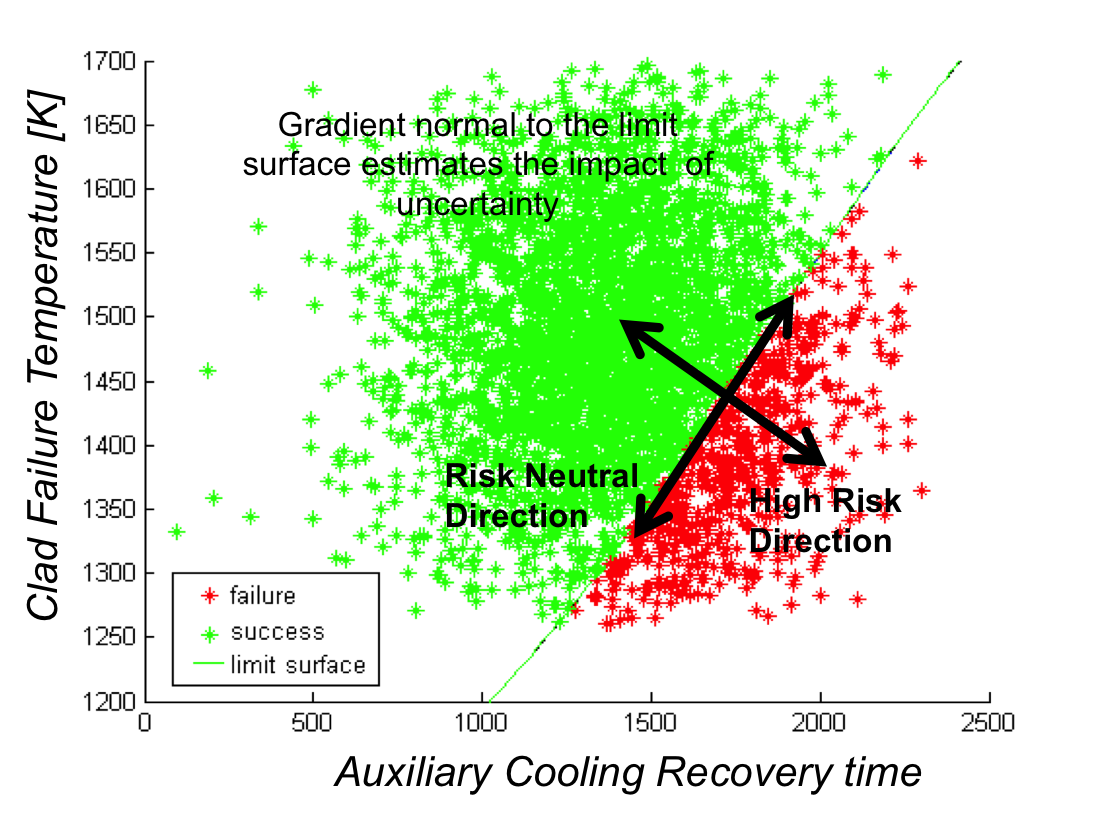
\includegraphics[width=1.0\textwidth]  {pics/ExampleLSwitRiskDirections.png}
  \caption{Example of limit surface highlighting the risk directions.}
  \label{fig:ExampleLSwitRiskDirections}
\end{figure}
In this case, the transition/failure probability is evaluated as follows:
\begin{equation}
\begin{matrix}
P_{F} = \bigintssss_{V_{F}}d\overline{x}\: pdf_{\overline{X}}\left ( \overline{x} \right )
= \bigintssss_{0}^{+\infty }d\overline{t_{F}}\: pdf_{T_{F}}\left ( T_{F} \right )\: \: \bigintssss_{\sqrt{\frac{t_{F}-t_{0}}{\alpha}}}^{+\infty } d\, rt_{DGs} \: pdf_{RT_{DGs}}\left ( rt_{DGs} \right )  =
\\
= \bigintssss_{t_{F_{min}}}^{t_{F_{max}}} dt_{F}\frac{1}{t_{F_{max}}-t_{F_{min}}}\: \: \bigintssss_{\sqrt{\frac{t_{F}-t_{0}}{\alpha}}}^{ rt_{DGs_{max}}}\: d\, rt_{DGs} \frac{1}{rt_{DGs_{max}}-rt_{DGs_{min}}} =
\\
= \frac{rt_{DGs_{max}}}{\Delta rt_{DGs}} + \frac{2\alpha}{3\left ( \Delta rt_{DGs}\Delta t_{F} \right )}
\left ( \sqrt[3/2]{\frac{t_{F_{min}}-t_{0}}{\alpha}} - \sqrt[3/2]{\frac{t_{F_{max}}-t_{0}}{\alpha}} \right )
\end{matrix}
\end{equation}

This simple example is useful to understand how the LS is defined in a practical application (that is analyzed numerically in the results Section) and how the hyper volume needs weighted with respect to the probability in the uncertain domain. An example of the computed LS is shown in Figure ~\ref{fig:ExampleLSwitRiskDirections}.
In this figure the neutral and high risk directions are highlighted.

%%%%%%%%%
%%%%%%%%% Limit Surface Search Algorithm
%%%%%%%%%
\paragraph{Limit Surface Search Algorithm}
\label{par:LSSalgorithm}
The identification of the LS location is extremely challenging,
depending on the particular physics/phenomena that are investigated.
To identify the real location of the LS, the evaluation of system
responses is needed, through the high-fidelity code (RELAP 7,
RELAP5-3D, etc.), in the full domain of uncertainty (infinite number of
combinations of uncertainties represented by the respective PDFs).
Obviously, this is not a feasible approach, and a reasonable
approximation is to locate the LS on a Cartesian N-D grid, in the
uncertain domain.

In reality, the location of the LS is not exactly determined but rather
bounded. The algorithm determines the set of grid nodes between
which the transition $0/1$ of the ``goal'' function happens. This set is
also classified with respect to the value of the ``goal'' function. With
reference to Figure~\ref{fig:LSgoalFunctionExample}, for example,
green is used for grid nodes with a
``goal'' function that equals $0$ and red when the ``goal'' function
equals $1$.
\begin{figure}[h!]
  \centering
  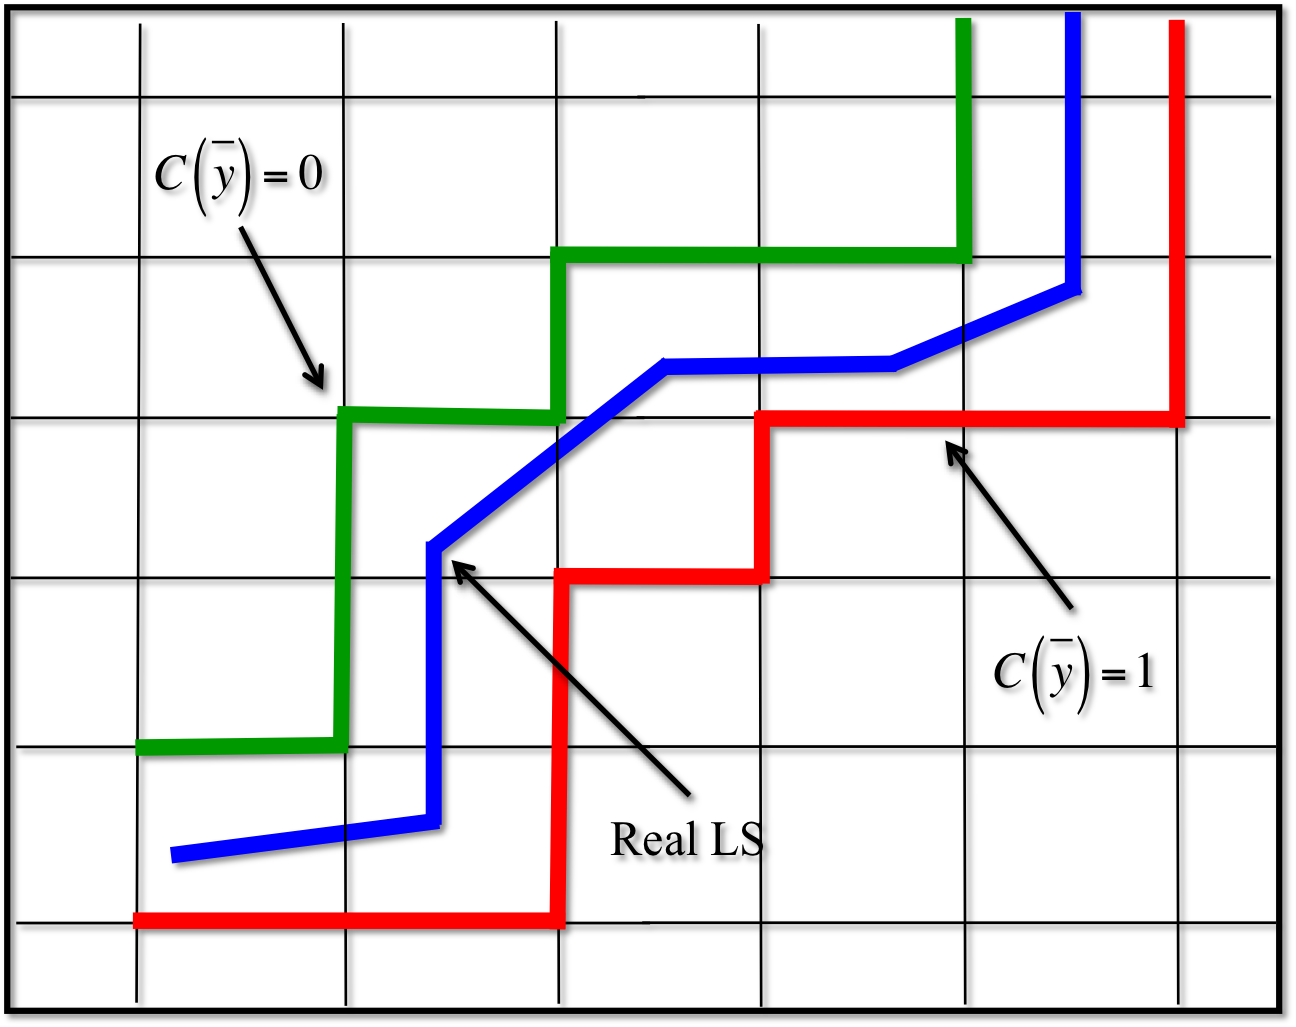
\includegraphics[width=1.0\textwidth]  {pics/LSgoalFunctionExample.png}
  \caption{Example of limit surface search evaluation grid (where $\overline{y}=\overline{\theta}$).}
  \label{fig:LSgoalFunctionExample}
\end{figure}
Each evaluation of the ``goal'' function in one of the grid nodes implies
the evaluation of the high-fidelity code (e.g. system simulator) for the
corresponding set of entries in the uncertain space. As already
mentioned, the evaluation of the high fidelity code is computationally
expensive and, in order to identify the LS, one should appraise
each point in the N-D grid covering the uncertainty space.
Discretization depends on the accuracy requested by the user. In
most cases, this approach is not feasible and, consequentially, the
process needs to be accelerated using ``predicting'' methods that are
represented by the employment of supervised learning algorithms
(i.e., ROMs).

This approach is commonly referred to as an active learning process
that ultimately results in training of a ROM of type classifier capable of
predicting the outcome of the ``goal'' function for any given point of
the uncertain space.
In an active learning process, a supervised learning algorithm is
combined with criteria to choose the next node in the N D grid that
needs explored, using the high fidelity physical model. This process is
repeated until, under a particular metric, the prediction capabilities of
the supervised learning algorithm do not improve by further increasing
the training set.

In more detail, the iterative scheme could be summarized through the following steps:
\begin{enumerate}
  \item A limited number of points in the uncertain space $\left \{
  \overline{x}_{k} \right \}$ are selected via one of the forward
  sampling strategies (e.g., stratified or Monte Carlo)
  \item The high fidelity code is used to compute the status of the
  system for the set of points in the input set:
  $
  \left \{ \overline{\theta}(t)\right \}_{k} = H\left ( \left \{ \overline{x} \right
  \}_{k},t \right )
  $.
  \item The ``goal'' function is evaluated at the phase space coordinate
  of the system:
  $\left \{ c \right \}_{k} = C\left ( \left \{ \overline{\theta}(t)\right \}_{k}
  \right )$
   \item The set of pairs $\left \{ \left ( \overline{x},c \right )_{k} \right \}$
   are used to train a ROM of type classifier, $G\left ( \left \{
   \overline{x}_{k} \right \} \right )$
   \item The ROM classifier is used to predict the values of the ``goal''
   function for all the $N$ nodes of the N-D grid in the domain space:
   \begin{equation}
   \left (G\left ( \left \{ \overline{x} \right \}_{j} \right ) \sim \left \{ c \right
   \}_{j}, j=1,...,N  \right )
    \end{equation}
    \item The values of the ``goal''  function are used to determine the
    LS location based on the change of values of  $\left \{ c \right
    \}_{j}$:
    \begin{equation}
    \left \{ c \right \}_{j}\rightarrow \partial V_{F}
     \end{equation}
     \item A new point is chosen to increase the training set and a new
     pair is generated
     \item The procedure is repeated starting from Step 3 until
     convergence is achieved. The convergence is achieved when
     there are no changes in the location of the LS after a certain
     number of consecutive iterations.
\end{enumerate}
The iteration scheme is graphically shown in
Figure~\ref{fig:LimitSurfaceAlgoFlow}.
\begin{figure}[h!]
  \centering
  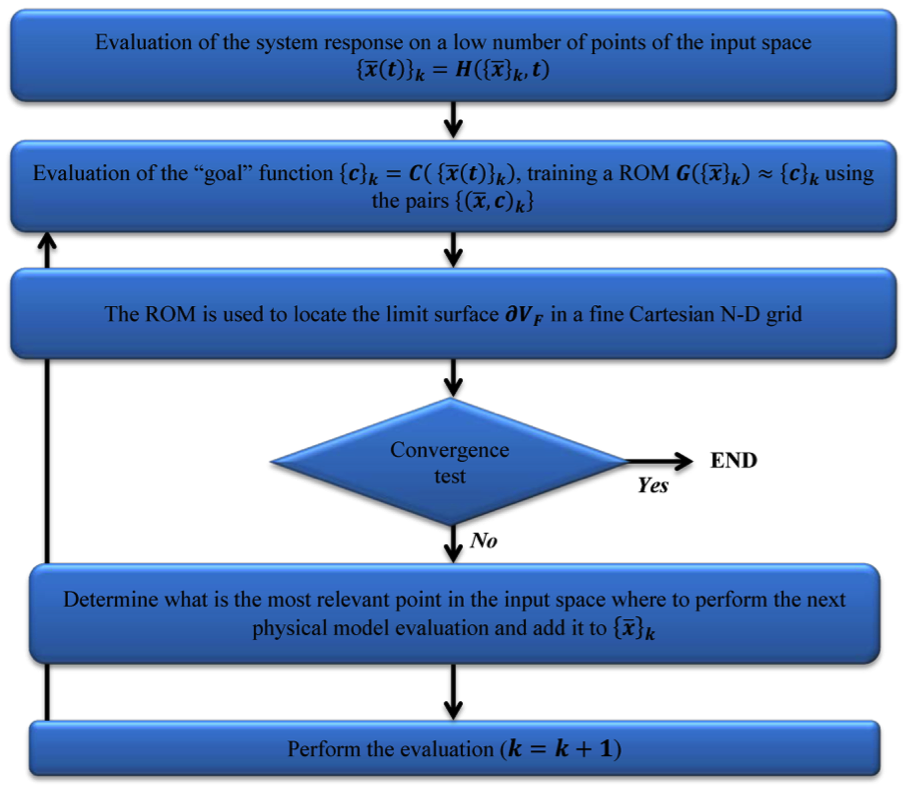
\includegraphics[width=1.0\textwidth]  {pics/LimitSurfaceAlgoFlow.png}
  \caption{Limit surface search algorithm conceptual scheme.}
  \label{fig:LimitSurfaceAlgoFlow}
\end{figure}
Note that there is an additional requirement
regarding the LS search algorithm:the LS location
has to stay constant for a certain number (user defined) of consecutive
iterations. The reason for this choice is determined by the attempt to
mitigate the effect of the build of non-linear bias in the searching
pattern. Indeed, the searching algorithm might focus too much on a
certain region of the LS while putting too few points in other zones
and completely hiding undiscovered topological features of the LS.
Regarding the strategy to choose the nodes on the N-D grid that
needs evaluated in the iterative process for the LS identification, it has
been decided to employ a metric based on the
distance between the predicted LS and the evaluations already
performed. The points on the LS are ranked based on the distance
from the closest training point already explored (the larger is the
distance the higher is the score for the candidate point), and based on
its persistence (the larger is the number of time the prediction of the
``goal'' function for that point have changed the higher is the score).
Since this approach creates a queue of ranked candidates, it could be
used also in the parallel implementation of the algorithm. When
several training points are run in parallel, it is possible that the
evaluation of one additional point does not alter dramatically the
location of the LS. Consequently, it is possible that the candidate with
the highest score is already being submitted for evaluation and
possibly the simulation is not yet completed. In this case, to avoid
submitting the same evaluation point twice, the algorithm searches
among all the ranked candidates (in descending order) for the one
that was not submitted for evaluation. Even if it is extremely unlikely
that all the candidates were submitted, in this remote event, the
method will choose the next point employing a Monte Carlo strategy.
%%%%%%%%%
%%%%%%%%% Acceleration through Multi-grid Approach
%%%%%%%%%
\paragraph{Acceleration through Multi-grid Approach}
\label{par:LSaccelerationMultiGrid}
The location of the LS, being a numerical iterative process, can be
known given a certain tolerance. As already mentioned, the LS search
is done by constructing an evaluation grid on which the acceleration
ROM is inquired. The tolerance of the iterative process determines how
the evaluation grid is discretized. Before addressing the acceleration
scheme, it is important
to introduce some concepts on the employed numerical process.
\begin{figure}[h!]
  \centering
  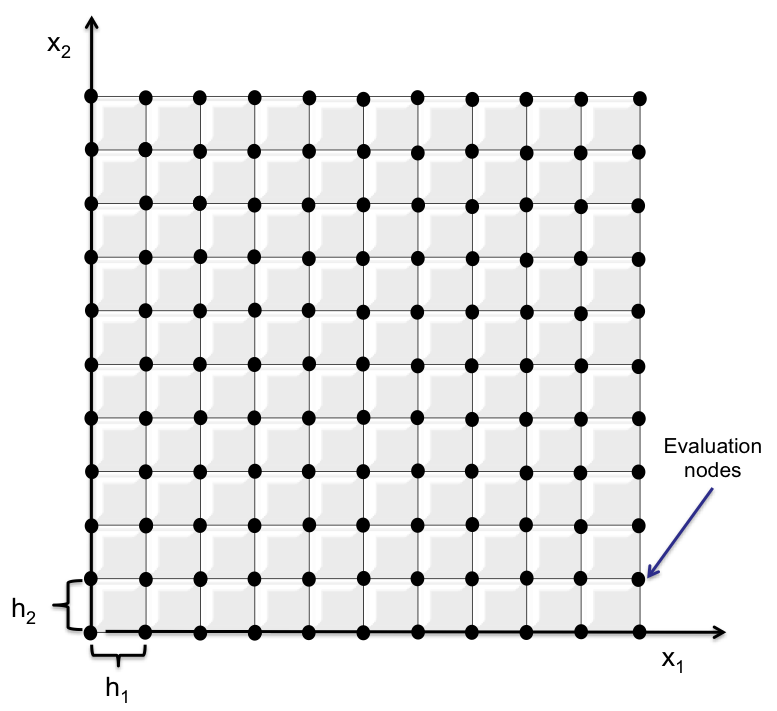
\includegraphics[width=1.0\textwidth]  {pics/DiscretizationGrid.png}
  \caption{Discretization grid.}
  \label{fig:DiscretizationGrid}
\end{figure}
\\Assume that each of $D$ dimensions of the uncertain domain is
discretized with the same number of equally-spaced nodes $N$ (see
Figure~\ref{fig:DiscretizationGrid}), with discretization size indicated
by $h_{i}$. Hence, the Cartesian grid contains $N^{D}$ individual
nodes, indexed through the multi-index vector $\overline{j} = \left (
j_{i=1\rightarrow D} \right ), j_{i} \leq N \forall i$. Introducing the
vectors  $\overline{I} = (1, ..., 1)$ and
$\overline{N} = (N, ..., N)$, the ``goal'' function is expressed on this N-
D grid as:
\begin{equation}
C\left ( \overline{x} \right ) =
\mathlarger{\sum}_{\overline{j}=\overline{I}}^{\overline{N}} \varphi_{\overline{j}}\left
( \overline{x} \right ) C\left ( \overline{x}_{\overline{j}} \right )
\end{equation}
where $\varphi_{\overline{j}}$ is the characteristic function of the hyper-volume $\Omega_{\overline{j}}$ surrounding the node
 $\overline{x}_{\overline{j}}$:
 \begin{equation}
 \varphi_{\overline{j}}\left ( \overline{x} \right ) =
\left\{\begin{matrix}
1 & if \: \overline{x} \in \Omega_{\overline{j}} \\
0 & if \: \overline{x} \notin \Omega_{\overline{j}}
\end{matrix}\right.
\end{equation}
where:
 \begin{equation}
 \label{eq:OmegaEq}
 \Omega_{\overline{j}} = \prod_{i=1}^{D}\left [ x_{j_{i}} - \frac{h_{i}}{2},
 x_{j_{i}} + \frac{h_{i}}{2}  \right ]
 \end{equation}
 The probability of the uncertain parameters is expressed as:
 \begin{equation}
 pdf_{\overline{X}}\left ( \overline{x} \right ) =
\mathlarger{\sum}_{\overline{j}=\overline{I}}^{\overline{N}}
\varphi_{\overline{j}}\left ( \overline{x} \right )
pdf_{\overline{X}}\left ( \overline{x}_{\overline{j}} \right )
 \end{equation}
Following the approach briefly explained in Section
\ref{sec:LSconcept}, the probability of the event (e.g., failure) could be
expressed as:
 \begin{equation}
 \label{eq:Pf}
  P_{F}=\left ( \prod_{i=1}^{D}h_{i} \right )
  \mathlarger{\sum}_{\overline{j}=
  \overline{I}}^{\overline{N}}pdf_{\overline{X}}\left (
  \overline{x_{\overline{j}}} \right )
  C\left ( \overline{x}_{\overline{j}} \right )
 \end{equation}
Under certain assumptions, the concept of active hyper-volume
$V_{A}$ as the region of the input space identified by the support of
the uncertain parameters’ probability density functions
$pdf_{\overline{X}}\left ( \overline{x} \right )$ could be introduced;
Equation ~\ref{eq:Pf} is recast, using a Taylor expansion, as follows:
 \begin{equation}
P_{F}= \bigintssss_{V} C\left ( \overline{x} \right )\: pdf_{\overline{X}}\left (
\overline{x}  \right )\: d\overline{x} =\bigintssss_{V_{A}}C\left ( \overline{x}
\right )\:
\left [
\mathlarger{\sum}_{\overline{j}=\overline{I}}^{\overline{N}}\varphi_{\overline{j}}\left (
\overline{x} \right )
\left ( pdf_{\overline{X}}\left ( \overline{x}_{\overline{j}} \right ) +
\mathlarger{\sum}_{i=1}^{D} \frac{\partial pdf_{\overline{X}}}{\partial x_{i}}|
_{\overline{x}_{\overline{j}}} \: \left ( x_{i} - x_{j_{i}} \right ) \right ) \right
] d\overline{x}
 \end{equation}
And, considering the evaluation grid as:
\begin{equation}
\label{eq:PfEq}
P_{F}= \mathlarger{\sum}_{\begin{matrix}
\overline{j}=\overline{I} \\ \overline{x}_{\overline{j}} \in V_{A} \end{matrix}}^{\overline{N}}
\bigintssss_{\overline{x}_{\overline{j}} - \overline{h}/2}^{\overline{x}_{\overline{j}} + \overline{h}/2} C\left ( \overline{x} \right )\:
\left [  \mathlarger{\sum}_{\overline{j}=\overline{I}}^{\overline{N}}\varphi_{\overline{j}}\left ( \overline{x} \right )
\left ( pdf_{\overline{X}}\left ( \overline{x}_{\overline{j}} \right ) +
\mathlarger{\sum}_{i=1}^{D} \frac{\partial pdf_{\overline{X}}}{\partial x_{i}}|_{\overline{x}_{\overline{j}}} \: \left ( x_{i} - x_{j_{i}} \right ) \right ) \right ] d\overline{x}
\end{equation}
At this point, it is possible to label, in the active hyper-volume, the sub-
domain identified by the nodes where the ``goal'' function
$C(\overline{x})$ changes its value (the frontier nodes between the
region where $C(\overline{x})=1$ and $C(\overline{x})=0$) $V_{A} \cap
V_{\partial V_{F}}$.
\\ Consequentially, it is possible to identify the sub-domains in which the  ``goal''  function $C(\overline{x})$ is equal to $0$ ($V_{A} \cap V_{\partial V_{C(\overline{x})=0}} \notin V_{A} \cap V_{\partial V_{F}}$):

\begin{equation}
\mathlarger{\sum}_{\begin{matrix}
\overline{j}=\overline{I} \\ \overline{x}_{\overline{j}} \in V_{A} \cap V_{C(\overline{x})=0} \end{matrix}}^{\overline{N}}
\bigintssss_{\overline{x}_{\overline{j}} - \overline{h}/2}^{\overline{x}_{\overline{j}} + \overline{h}/2} C\left ( \overline{x} \right )\:
\left ( pdf_{\overline{X}}\left ( \overline{x}_{\overline{j}} \right ) +
\mathlarger{\sum}_{i=1}^{D} \frac{\partial pdf_{\overline{X}}}{\partial x_{i}}|_{\overline{x}_{\overline{j}}} \: \left ( x_{i} - x_{j_{i}} \right ) \right )   d\overline{x}
\end{equation}
in which the  ``goal''  function $C(\overline{x})$ is equal to $1$ ($V_{A} \cap V_{\partial V_{C(\overline{x})=1}} \notin V_{A} \cap V_{\partial V_{F}}$):
\begin{equation}
\begin{matrix}
\mathlarger{\sum}_{\begin{matrix}
\overline{j}=\overline{I} \\ \overline{x}_{\overline{j}} \in V_{A} \cap V_{C(\overline{x})=1} \end{matrix}}^{\overline{N}}
\bigintssss_{\overline{x}_{\overline{j}} - \overline{h}/2}^{\overline{x}_{\overline{j}} + \overline{h}/2} C\left ( \overline{x} \right )\:
\left ( pdf_{\overline{X}}\left ( \overline{x}_{\overline{j}} \right ) +
\mathlarger{\sum}_{i=1}^{D} \frac{\partial pdf_{\overline{X}}}{\partial x_{i}}|_{\overline{x}_{\overline{j}}} \: \left ( x_{i} - x_{j_{i}} \right ) \right )   d\overline{x} =
\\
= \mathlarger{\sum}_{\begin{matrix}
\overline{j}=\overline{I} \\ \overline{x}_{\overline{j}} \in V_{A} \cap V_{C(\overline{x})=1} \end{matrix}}^{\overline{N}}
\bigintssss_{\overline{x}_{\overline{j}} - \overline{h}/2}^{\overline{x}_{\overline{j}} + \overline{h}/2}
\left ( pdf_{\overline{X}}\left ( \overline{x}_{\overline{j}} \right ) +
\mathlarger{\sum}_{i=1}^{D} \frac{\partial pdf_{\overline{X}}}{\partial x_{i}}|_{\overline{x}_{\overline{j}}} \: \left ( x_{i} - x_{j_{i}} \right ) \right )   d\overline{x}
\end{matrix}
\end{equation}
Equation ~\ref{eq:PfEq} is now expressed as:
 \begin{equation}
 \label{eq:PfEqFinal}
 \begin{matrix}
P_{F} = \mathlarger{\sum}_{\begin{matrix}
\overline{j}=\overline{I} \\ \overline{x}_{\overline{j}} \in V_{A} \cap
V_{C(\overline{x})=1} \end{matrix}}^{\overline{N}}
\left ( \prod_{i=1}^{D}
 h_{i} \right )
\: pdf_{\overline{X}} ( \overline{x}_{\overline{j}}) + O(h^{N+1}) +
 \\
 + \mathlarger{\sum}_{\begin{matrix}
\overline{j}=\overline{I} \\ \overline{x}_{\overline{j}} \in V_{A} \cap
V_{\partial V_{f}} \end{matrix}}^{\overline{N}}
\bigintssss_{\overline{x}_{\overline{j}} -
\overline{h}/2}^{\overline{x}_{\overline{j}} + \overline{h}/2} C\left (
\overline{x} \right )\: \left ( pdf_{\overline{X}}\left (
\overline{x}_{\overline{j}} \right ) +
\mathlarger{\sum}_{i=1}^{D} \frac{\partial pdf_{\overline{X}}}{\partial
x_{i}}|_{\overline{x}_{\overline{j}}} \: \left ( x_{i} - x_{j_{i}} \right ) \right )
d\overline{x}
\end{matrix}
 \end{equation}
As inferred from Equation ~\ref{eq:PfEqFinal}, the process is bounded if the
surface area-to-volume ratio (amount of surface area per unit volume) is
in favor of the volume:
\begin{equation}
\label{eq:convergenceCondition}
\mathlarger{\sum}_{\begin{matrix}
\overline{j}=\overline{I} \\ \overline{x}_{\overline{j}} \in V_{A} \cap
V_{C(\overline{x})=1} \end{matrix}}^{\overline{N}}
\left ( \prod_{i=1}^{D}
 h_{i} \right )
\: pdf_{\overline{X}} ( \overline{x}_{\overline{j}})
\gg
\sum_{\begin{matrix}
\overline{j}=\overline{I} \\ \overline{x}_{\overline{j}} \in V_{A} \cap
V_{\partial V_{f}} \end{matrix}}^{\overline{N}}
\left | \int_{\overline{x}_{\overline{j}} -
\overline{h}/2}^{\overline{x}_{\overline{j}} + \overline{h}/2}   pdf_{\overline{X}}\left (
\overline{x}_{\overline{j}} \right )  \right |
d\overline{x}
\end{equation}
If the grid is built in the transformed space of probability (i.e., replacing the measure $d\overline{x}$ with $d \overline{\mu }\: \: pdf_{\overline{X}}\left ( \overline{x}_{\overline{j}} \right )$ the condition expressed in Equation ~\ref{eq:convergenceCondition} is reduced:
\begin{equation}
number \: \:  nodes \in V_{A} \cap V_{C(\overline{x})=1} \gg number \: \:  nodes  \in V_{A} \cap V_{\partial V_{F}}
\end{equation}
This means that error is bounded by the total probability contained in the cells on the frontier of the LS.

Based on this derivation, it is clear how important it is to keep the
content of the total probability on the frontier of the LS as low as
possible, and simultaneously, increase the importance of the volume of
the failure/event region as much as possible (to improve the surface
area-to-volume ratio).

To do that, the step size in probability should be significantly
reduced ( $h_{i}^{p} \rightarrow 0^{+}$). Even if this is theoretically
feasible, it is computational inapplicable. To approach a similar result, it
is possible to learn from other numerical methods that use the
technique of adaptive meshing for the resolution of the partial
differential equation system (e.g., finite element methods).

For this reason, an acceleration scheme was designed and developed
employing a multi-grid approach. The main idea, it is to recast the
iterative process in two different sub-sequential steps. Firstly,
performing the LS search on a coarse evaluation grid, and once
converged, adaptively refining the cells that lie on the frontier of the LS
($V_{A} \cap V_{\partial V_{F}}$) and, consequentially, converging on
the new refined grid.
\\The iteration scheme is graphically shown in
Figure~\ref{fig:LimitSurfaceMultiGridAlgoFlow}.
\begin{figure}[h!]
  \centering
  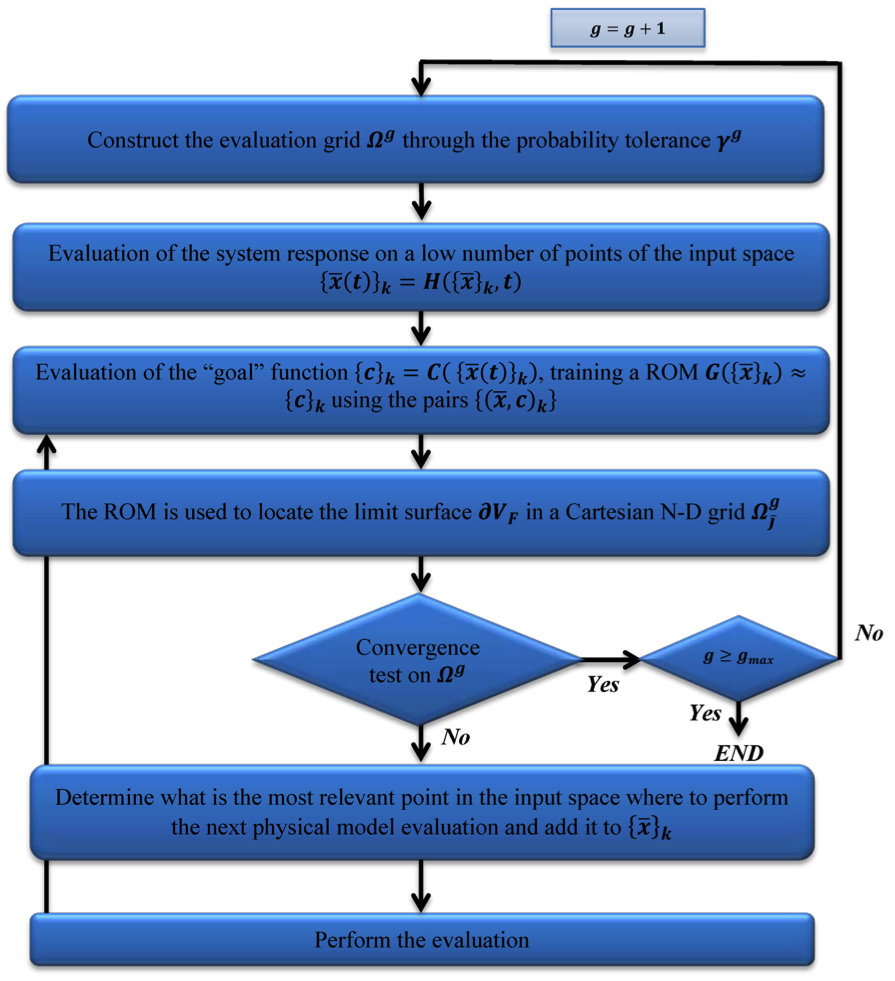
\includegraphics[width=1.0\textwidth]  {pics/LimitSurfaceMultiGridAlgoFlow.png}
  \caption{Multi-grid limit surface search scheme.}
  \label{fig:LimitSurfaceMultiGridAlgoFlow}
\end{figure}
In more detail, the iterative scheme could be summarized through the
following steps:
\begin{enumerate}
  \item The user specifies two tolerances in probability $(CDF):
  \gamma^{g=1}$ for the initial coarse grid and $\gamma^{g=2}$
  for the refined grid, where  $ \gamma^{g=1} >  \gamma^{g=2}$;
  \item Following Equation ~\ref{eq:OmegaEq}, the initial coarse evaluation
  grid $\Omega^{1}$ is constructed ($N^{g=1}$ total nodes). The
  discretization of this grid is done to have cells with a content of
  probability equal to $\gamma^{g=1}$.
  \item A limited number of points in the uncertain space $\left \{
  \overline{x}_{k} \right \}$ are selected via one of the forward
  sampling strategies (e.g., stratified or Monte Carlo).
  \item The high fidelity code is used to compute the status of the
  system for the set of points in the input set:
  $
  \left \{ \overline{\theta}(t)\right \}_{k} = H\left ( \left \{ \overline{x} \right
  \}_{k},t \right )
  $.
  \item The ``goal'' function is evaluated at the phase space coordinate
  of the system:
  $\left \{ c \right \}_{k} = C\left ( \left \{ \overline{\theta}(t)\right \}_{k}
  \right )$.
   \item The set of pairs $\left \{ \left ( \overline{x},c \right )_{k} \right \}$
   are used to train a ROM of type classifier, $G\left ( \left \{
   \overline{x}_{k} \right \} \right )$.
   \item The ROM classifier is used to predict the values of the ``goal''
   function for all the $N^{g=1}$ nodes of the N-D grid in the domain
   space:
   \begin{equation}
   \left (G\left ( \left \{ \overline{x} \right \}_{j} \right ) \sim \left \{ c \right
   \}_{j}, j=1,...,N^{g=1}  \right )
    \end{equation}
    \item The values of the ``goal''  function are used to determine the
    LS location based on the change of values of  $\left \{ c \right
    \}_{j}$:
    \begin{equation}
    \left \{ c \right \}_{j}\rightarrow \partial V_{F}
     \end{equation}
     \item A new point is chosen to increase the training set and a new
     pair is generated.
     \item The procedure is repeated starting from Step 5 until
     convergence is achieved on grid $\Omega^{g}$.The convergence
     is reached when there are no changes in the location of the LS
     after a certain number of consecutive iterations (user defined).
     \item When the convergence is achieved on the coarse grid
     $\Omega^{g=1}$, all the cells that lie on the frontier of the LS
     ($V_{A} \cap V_{\partial V_{F}}$) are refined to contain an amount of
     probability equal to  $\gamma^{g=2}$.
     \item Steps 7 through 9 are performed based on the new refined
     grid. Finally, the process starts again by performing Steps 5
     through 10, until the convergence is achieved in the refined grid.
\end{enumerate}
As shown in Figure~\ref{fig:LimitSurfaceMultiGridAlgoFlow}, the
algorithm consists in searching the location of the LS proceeding with
subsequential refinement of the sub-domain, in the active space, that
contains the LS. In this way, the computational burden is kept as low as
possible. In addition, another advantage of this approach is that, since
the refinement grid represents a constrained domain, the sub-
sequential ROM training process can be regularized, since the LS
between an iteration and the other can move, at maximum, within the
refinement domain.

%%%%%%%%%%%%%%%%
\subsubsection{Limit Surface Search sampling through RAVEN}
\label{subsub:LSsamplingExample}
The goal of this Section is to learn how to:
 \begin{enumerate}
   \item Set up a LS Search sampling for efficiently perturb a driven code
   \item Use the LS Integral Post-processor for computing the probability of failure of the system subject to the same
   ``goal'' function
   \item Plot the obtained LS.
\end{enumerate}
In order to accomplish these tasks, the following RAVEN \textbf{Entities} (XML blocks in the input files) are defined:
\begin{enumerate}
   \item \textbf{\textit{RunInfo}}:
\begin{lstlisting}[style=XML,morekeywords={arg,extension,pauseAtEnd,overwrite}]
  <RunInfo>
    <JobName>LSsearch</JobName>
    <Sequence>
      sample,computeLSintegral,writeHistories
    </Sequence>
    <WorkingDir>LSsearch</WorkingDir>
    <batchSize>8</batchSize>
  </RunInfo>
\end{lstlisting}
   As shown in Section~\ref{sub:EntitiesAndFlow}, the \textit{RunInfo} \textbf{Entity} is intended to set up the analysis
   that the user wants to perform. In this specific case, three steps (\xmlNode{Sequence}) are  sequentially run
   using eight processors (\xmlNode{batchSize}).
   \item \textbf{\textit{Files}}:
\begin{lstlisting}[style=XML,morekeywords={arg,extension,pauseAtEnd,overwrite}]
  <Files>
    <Input name="referenceInput.xml" type="input">referenceInput.xml</Input>
    <Input name="LSintegral.csv" type="">LSintegral.csv</Input>
  </Files>
\end{lstlisting}
   Since the driven code uses a single input file, in this Section the original input is placed. As detailed in the user manual
   the attribute  \xmlAttr{name} represents the alias that is going to be
   used in all the other input blocks in order to refer to this file.
   \\In addition the output file used in \xmlNode{Sequence}
   \textit{computeLSintegral} is here inputted.
   \item \textbf{\textit{Models}}:
\begin{lstlisting}[style=XML,morekeywords={arg,extension,pauseAtEnd,overwrite}]
  <Models>
    <Code name="testModel" subType="GenericCode">
      <executable>
      ../physicalCode/analyticalbateman/AnalyticalDplMain.py
      </executable>
      <clargs arg="python" type="prepend"/>
      <clargs arg="" extension=".xml" type="input"/>
      <clargs arg="" extension=".csv" type="output"/>
      <prepend>python</prepend>
    </Code>
    <ROM name="AccelerationROM" subType="SciKitLearn">
      <Features>sigma-A,decay-A</Features>
      <Target>goalFunction</Target>
      <SKLtype>neighbors|KNeighborsClassifier</SKLtype>
      <n_neighbors>1</n_neighbors>
    </ROM>
    <PostProcessor name="integralLS" subType="LimitSurfaceIntegral">
      <tolerance>0.001</tolerance>
      <integralType>MonteCarlo</integralType>
      <seed>20021986</seed>
      <target>goalFunction</target>
      <variable name="sigma-A">
        <distribution>sigmaA</distribution>
      </variable>
      <variable name="decay-A">
        <distribution>decayConstantA</distribution>
      </variable>
    </PostProcessor>
  </Models>
\end{lstlisting}
 As mentioned above, the goal of this example is the employment of
 an efficient sampling strategy, having as goal the determination of the
 failure of a system.

 In addition to the previously explained Code
 model,
 the ROM of type \textit{SciKitLearn} is here specified. The ROM will be
 used in the adaptive sampling strategy \textit{LimitSurfaceSearch} in
 order to accelerate the convergence of the method. As it can be seen,
 a nearest neighbor classifier is used, targeting only two uncertainties
 $sigma-A and decay-A$.
 \\ For the computation of the probability of failure (see the following), a
 Post-Processor (PP) of type \textit{LimitSurfaceIntegral} is here
 specified.This PP performs an integral of the LS
 generated by the adaptive sampling technique.
   \item \textbf{\textit{Distributions}}:
\begin{lstlisting}[style=XML]
  <Distributions>
      <Uniform name="sigmaA">
          <lowerBound>0</lowerBound>
          <upperBound>1000</upperBound>
      </Uniform>
      <Uniform name="decayConstantA">
          <lowerBound>0.00000001</lowerBound>
          <upperBound>0.0000001</upperBound>
      </Uniform>
  </Distributions>
\end{lstlisting}
  In the Distributions XML Section, the stochastic model for the
  uncertainties  treated by the LS search sampling are reported. In
  this case two distributions are defined:
  \begin{itemize}
    \item $sigmaA \sim \mathbb{U}(0,1000)$, used to model the uncertainty
    associated with  the Model \textit{sigma-A}
    \item  $decayConstantA \sim \mathbb{U}(1e-8,1e-7)$,  used to
    model the uncertainty
    associated with  the Model \textit{decay-A}.
  \end{itemize}
   \item \textbf{\textit{Samplers}}:
\begin{lstlisting}[style=XML,morekeywords={arg,extension,pauseAtEnd,overwrite}]
  <Samplers>
    <LimitSurfaceSearch name="LSsearchSampler">
      <ROM              class="Models"      type="ROM">AccelerationROM</ROM>
      <Function         class="Functions"   type="External">goalFunction</Function>
      <TargetEvaluation class="DataObjects" type="PointSet">samples</TargetEvaluation>
      <Convergence forceIteration="False" limit="50000" persistence="20"  weight="CDF">0.00001</Convergence>
      <variable name="sigma-A">
        <distribution>sigmaA</distribution>
      </variable>
      <variable name="decay-A">
        <distribution>decayConstantA</distribution>
      </variable>
    </LimitSurfaceSearch>
  </Samplers>
\end{lstlisting}
  In order to employ the LS search sampling strategy, a
  \xmlNode{LimitSurfaceSearch} node needs to be inputted.
  As it can be
  seen from above, each variable is associated to a different distribution
  defined in the  \xmlNode{Distributions} block.
  In addition, the \textit{AccelerationROM}  \xmlNode{ROM} is inputted.
  As already mentioned, this ROM (of type classifier) is used to
  accelerate the convergence of the LS Search method.
  In addition, the goal function \textit{goalFunction}  and the
  \textit{samples} are here reported.
  \\For this example, a convergence criterion of $1.0e-5$ is set. To reach such a confidence with a Monte-Carlo, millions of
  samples would be needed.
   \item \textbf{\textit{Functions}}:
\begin{lstlisting}[style=XML,morekeywords={arg,extension,pauseAtEnd,overwrite}]
 <Functions>
   <External file="goalFunction" name="goalFunction">
     <variable>A</variable>
   </External>
 </Functions>
\end{lstlisting}
 As already mentioned, the LS search sampling strategy uses
 a goal function in order to identify the regions of the uncertain space
 that are more informative. The \textit{goalFunction} used for this
 example is reported below. As it can be seen, if the final response $A$
 is $<=$ of $0.3$ , the system is considered to be in a ``safe'' condition.
\begin{lstlisting}[language=python]
def __residuumSign(self):
  returnValue = 1.0
  if self.A  <= 0.3:
    returnValue = -1.0
  return returnValue
\end{lstlisting}

   \item \textbf{\textit{DataObjects}}:
\begin{lstlisting}[style=XML,morekeywords={arg,extension,pauseAtEnd,overwrite}]
  <DataObjects>
    <PointSet name="limitSurface">
      <Input>sigma-A,decay-A</Input>
      <Output>goalFunction</Output>
    </PointSet>
    <PointSet name="samples">
      <Input>sigma-A,decay-A</Input>
      <Output>A,B,C,D,time</Output>
    </PointSet>
    <HistorySet name="histories">
      <Input>sigma-A,decay-A</Input>
      <Output>A,B,C,D,time</Output>
    </HistorySet>
  </DataObjects>
\end{lstlisting}
  In this block, three \textit{DataObjects} are defined: 1) PointSet
  named ``samples'' used to collect the final outcomes of the code, 2)
  HistorySet named ``histories'' in which the full time responses of the
  variables $A,B,C,D$ are going to be stored, 3) PointSet named
  ``limitSurface'' used  to export the LS location (in the uncertain space) during the employment of the sampling strategy.
 %%%%%%%%%%%%%%%%%%%%%%%%%%%%%%%%%%%%%%%%%%%%%%%%%%%%%%%%%%
 %%%%%%%%%%%%%%%%%%%%%%%%%%%%%%%%%%%%%%%%%%%%%%%%%%%%%%%%%%
 %figure samples
 \begin{figure}[h!]
  \centering
  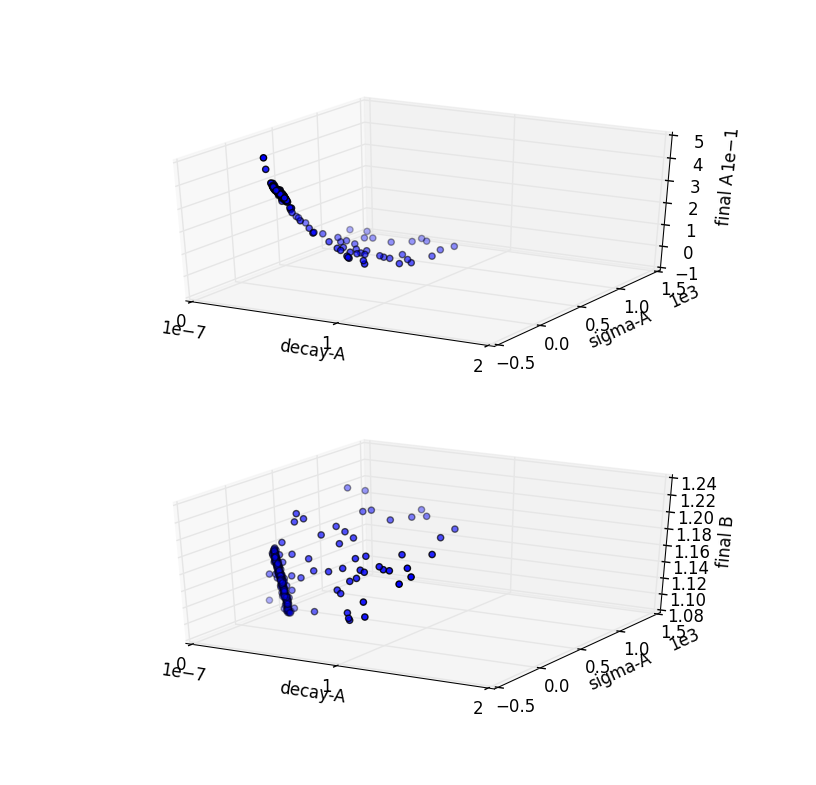
\includegraphics[scale=0.7]{pics/LS_pointsets.png}
  \caption{Plot of the samples generated by the LS search sampling for variables $A,B$.}
  \label{fig:LS_pointsets}
 \end{figure}
 %%%%%%%%%%%%%%%%%%%%%%%%%%%%%%%%%%%%%%%%%%%%%%%%%%%%%%%%%%
 %%%%%%%%%%%%%%%%%%%%%%%%%%%%%%%%%%%%%%%%%%%%%%%%%%%%%%%%%%
   \item \textbf{\textit{Steps}}:
\begin{lstlisting}[style=XML,morekeywords={arg,extension,pauseAtEnd,overwrite}]
  <Steps>
    <MultiRun name="sample">
      <Input          class="Files"       type="input">referenceInput.xml</Input>
      <Model          class="Models"      type="Code">testModel</Model>
      <Sampler        class="Samplers"    type="LimitSurfaceSearch">LSsearchSampler</Sampler>
      <SolutionExport class="DataObjects" type="PointSet">limitSurface</SolutionExport>
      <Output         class="DataObjects" type="PointSet">samples</Output>
      <Output         class="DataObjects" type="HistorySet">histories</Output>
    </MultiRun>
    <PostProcess name="computeLSintegral">
      <Input  class="DataObjects" type="PointSet"     >limitSurface</Input>
      <Model  class="Models"      type="PostProcessor">integralLS</Model>
      <Output class="DataObjects" type="PointSet"     >limitSurface</Output>
      <Output class="Files"       type=""             >LSintegral.csv</Output>
    </PostProcess>
    <IOStep name="writeHistories" pauseAtEnd="True">
      <Input  class="DataObjects"      type="HistorySet">histories</Input>
      <Input  class="DataObjects"      type="PointSet">samples</Input>
      <Input  class="DataObjects"      type="PointSet">limitSurface</Input>
      <Output class="OutStreamManager" type="Plot">samplesPlot3D</Output>
      <Output class="OutStreamManager" type="Plot">historyPlot</Output>
      <Output class="OutStreamManager" type="Print">samples</Output>
      <Output class="OutStreamManager" type="Plot">limitSurfacePlot</Output>
      <Output class="OutStreamManager" type="Print">histories</Output>
    </IOStep>
  </Steps>
\end{lstlisting}
  %%%%%%%%%%%%%%%%%%%%%%%%%%%%%%%%%%%%%%%%%%%%%%%%%%%%%%%%%%
 %figure samples
 \begin{figure}[h!]
  \centering
  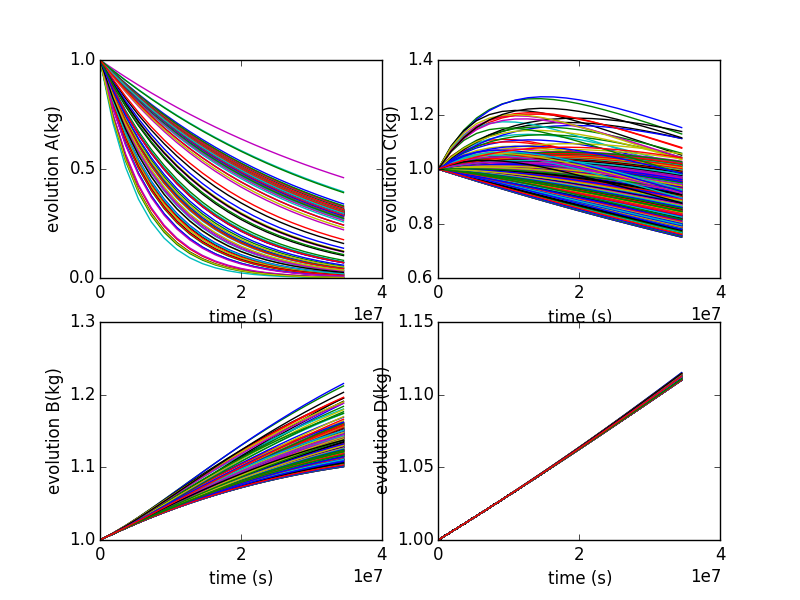
\includegraphics[scale=0.7]{pics/LS_histories.png}
  \caption{Plot of the histories generated by the LS search method for variables $A,B,C,D$.}
  \label{fig:LS_histories}
 \end{figure}
 %%%%%%%%%%%%%%%%%%%%%%%%%%%%%%%%%%%%%%%%%%%%%%%%%%%%%%%%%%
   Finally, all the previously defined \textbf{Entities} can be combined in
   the \xmlNode{Steps} block. As inferable,
   three \xmlNode{Steps} have been inputted:
   \begin{itemize}
     \item \xmlNode{MultiRun} named ``sample'', used to run the multiple
     instances of the driven code and
     collect the outputs in the two \textit{DataObjects}. As it can be
     seen, the \xmlNode{Sampler} is inputted to communicate to the
     \textit{Step} that the driven code needs to
     be perturbed through the LS search sampling strategy;
     \item \xmlNode{PostProcess} named ``computeLSintegral'', used to
     compute the probability of failure of the system based on the LS generated employing the LS search strategy. This
     probability is computed integrating the LS with a Monte-Carlo
     method.
     \item  \xmlNode{IOStep} named ``writeHistories'', used to 1) export
     the ``histories'' and ``samples''  \textit{DataObjects}
     \textbf{Entity} in a CSV file and 2) plot the data and the Limit Surface
     in  PNG files and on the screen.
   \end{itemize}
\end{enumerate}
 Figure~\ref{fig:LS_histories}
 shows the evolution of the outputs $A,B,C,D$ under uncertainties.
 Figure~\ref{fig:LS_pointsets} shows the final responses  of $A and B$
 of the sampling employed using the driven code.
 Figure~\ref{fig:LSplot}  shows the limit surface for this particular
 example. Only $367$ samples were needed in order to reach the full
 convergence.
 \\The integration of the LS determines a probability of failure of
 $~3.45e-2$.
  %%%%%%%%%%%%%%%%%%%%%%%%%%%%%%%%%%%%%%%%%%%%%%%%%%%%%%%%%%
 %figure samples
 \begin{figure}[h!]
  \centering
  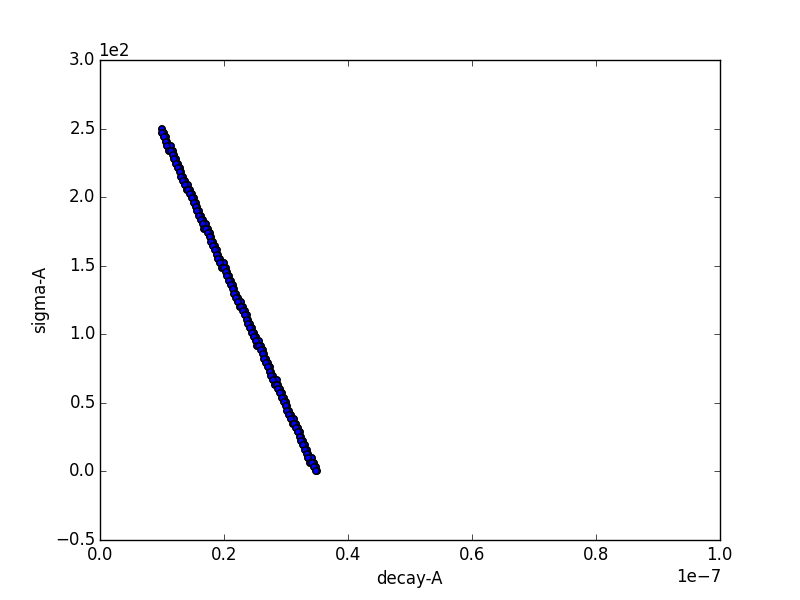
\includegraphics[scale=0.7]{pics/LimitSurfacePlot.png}
  \caption{Limit Surface generated by the LS search method.}
  \label{fig:LSplot}
 \end{figure}
 %%%%%%%%%%%%%%%%%%%%%%%%%%%%%%%%%%%%%%%%%%%%%%%%%%%%%%%%%%








